\documentclass[12pt,a4paper]{article}

% ── Packages ──────────────────────────────────────────────────────────────────
\usepackage[a4paper, margin=2.4cm]{geometry}
\usepackage[T1]{fontenc}
\usepackage[utf8]{inputenc}
\usepackage{lmodern}
\usepackage{microtype}
\usepackage{graphicx}
\usepackage{amsmath, amssymb}
\usepackage{booktabs}
\usepackage{array}
\usepackage{tabularx}
\usepackage{xcolor}
\usepackage{listings}
\usepackage{caption}
\usepackage{subcaption}
\usepackage{float}
\usepackage{hyperref}
\usepackage{titlesec}
\usepackage{enumitem}
\usepackage{parskip}
\usepackage{fancyhdr}
\usepackage[most]{tcolorbox}

% ── Graphics path ─────────────────────────────────────────────────────────────
\graphicspath{{./images/}}

% ── Colours ───────────────────────────────────────────────────────────────────
\definecolor{darkblue}{RGB}{0,51,102}
\definecolor{steelblue}{RGB}{70,130,180}
\definecolor{lightgray}{RGB}{245,245,245}
\definecolor{codegray}{RGB}{240,240,240}
\definecolor{codered}{RGB}{163,21,21}
\definecolor{codegreen}{RGB}{0,128,0}
\definecolor{codeblue}{RGB}{0,0,205}

% ── Hyperref ──────────────────────────────────────────────────────────────────
\hypersetup{
    colorlinks=true, linkcolor=darkblue,
    urlcolor=steelblue, citecolor=darkblue,
    pdftitle={Lab 06 -- Anomaly Detection using VAE and GAN},
    pdfauthor={CS23B1028 R K Larika, CS23B1050 S Harshini}
}

% ── Section styles ────────────────────────────────────────────────────────────
\titleformat{\section}{\Large\bfseries\color{darkblue}}{}{0em}{}[\titlerule]
\titleformat{\subsection}{\large\bfseries\color{steelblue}}{}{0em}{}
\titleformat{\subsubsection}{\normalsize\bfseries\color{darkblue}}{}{0em}{}

% ── Code listing ──────────────────────────────────────────────────────────────
\lstset{
    language=Python,
    backgroundcolor=\color{codegray},
    basicstyle=\footnotesize\ttfamily,
    keywordstyle=\color{codeblue}\bfseries,
    stringstyle=\color{codered},
    commentstyle=\color{codegreen}\itshape,
    numberstyle=\tiny\color{gray},
    numbers=left, numbersep=8pt, stepnumber=1,
    frame=single, framesep=5pt,
    rulecolor=\color{steelblue},
    breaklines=true, showstringspaces=false,
    tabsize=4, captionpos=b,
    xleftmargin=1.5em, aboveskip=8pt, belowskip=8pt
}

% ── Header / Footer ───────────────────────────────────────────────────────────
\pagestyle{fancy}
\fancyhf{}
\fancyhead[L]{\small\textcolor{darkblue}{\textbf{Lab 06 -- Anomaly Detection using VAE \& GAN}}}
\fancyhead[R]{\small\textcolor{gray}{Deep Learning Lab}}
\fancyfoot[C]{\thepage}
\renewcommand{\headrulewidth}{0.4pt}
\renewcommand{\headrule}{\hbox to\headwidth{\color{steelblue}\leaders\hrule height\headrulewidth\hfill}}

% ── tcolorbox styles ──────────────────────────────────────────────────────────
\newtcolorbox{notebox}{
    enhanced, breakable,
    colback=lightgray, colframe=steelblue,
    fonttitle=\bfseries, title=Note,
    arc=3pt, boxrule=0.8pt,
    left=6pt, right=6pt, top=4pt, bottom=4pt
}
\newtcolorbox{keybox}{
    enhanced, breakable,
    colback=yellow!10!white, colframe=darkblue,
    fonttitle=\bfseries\color{white}, title=Key Takeaway,
    colbacktitle=darkblue,
    arc=3pt, boxrule=0.8pt,
    left=6pt, right=6pt, top=4pt, bottom=4pt
}

% ══════════════════════════════════════════════════════════════════════════════
\begin{document}

% ── Title Page ────────────────────────────────────────────────────────────────
\begin{titlepage}
\centering
\vspace*{1.8cm}

{\color{darkblue}\rule{\linewidth}{2pt}}
\vspace{0.9cm}

{\Huge\bfseries\color{darkblue}
    Anomaly Detection using\\[0.4em]
    Variational Autoencoder (VAE)\\[0.4em]
    and Generative Adversarial Network (GAN)
}

\vspace{0.7cm}
{\color{steelblue}\rule{\linewidth}{1pt}}
\vspace{1.2cm}

{\LARGE\bfseries Lab Report --- Lab 06}

\vspace{0.4cm}
{\large Deep Learning Laboratory}

\vspace{1.8cm}

\begin{tabular}{rl}
    \textbf{Students:}   & CS23B1028 \quad R K Larika \\[4pt]
                         & CS23B1050 \quad S Harshini  \\[12pt]
    \textbf{Dataset:}    & LGG MRI Segmentation (Kaggle -- mateuszbuda) \\[4pt]
    \textbf{Platform:}   & Kaggle GPU (NVIDIA T4) \\[4pt]
    \textbf{Framework:}  & PyTorch 2.x \\[4pt]
    \textbf{Date:}       & \today
\end{tabular}

\vfill
{\color{darkblue}\rule{\linewidth}{2pt}}
\end{titlepage}

% ── Table of Contents ─────────────────────────────────────────────────────────
\tableofcontents
\newpage

% ══════════════════════════════════════════════════════════════════════════════
\section{Introduction and Objective}

Anomaly detection in medical imaging is a high-stakes problem where the goal is to identify
pathological regions (e.g.\ brain tumours) \textit{without} requiring pixel-level annotations
during training.  A powerful unsupervised strategy trains a generative model exclusively on
\emph{normal} (healthy) scans and then exploits the model's inability to faithfully reconstruct
\emph{abnormal} (tumour-containing) anatomy as an anomaly signal.

This lab explores and compares two state-of-the-art generative architectures for this purpose:

\begin{enumerate}[leftmargin=1.6cm]
    \item \textbf{Variational Autoencoder (VAE)} --- a probabilistic encoder-decoder that
          learns a smooth, Gaussian-regularised latent space.
    \item \textbf{Encoder-Decoder Generator (GAN)} --- a U-Net style generator adversarially
          trained with a PatchGAN discriminator.
\end{enumerate}

Both models are trained \textbf{only on normal MRI slices}.  At inference time, an abnormal
slice is poorly reconstructed; the pixel-wise absolute difference between the original and its
reconstruction produces a \emph{Region-of-Interest (ROI)} mask that localises the tumour.

% ══════════════════════════════════════════════════════════════════════════════
\section{Dataset and Preprocessing}
\label{sec:data}

\subsection{Dataset Description}

The experiment uses the \textbf{LGG MRI Segmentation} dataset
(\texttt{mateuszbuda/lgg-mri-segmentation}) available on Kaggle.  It contains brain MRI slices
from patients with Low-Grade Glioma (LGG) alongside binary segmentation masks that delineate
tumour regions.

\begin{table}[H]
\centering
\caption{Dataset Statistics}
\label{tab:dataset}
\begin{tabular}{lcc}
\toprule
\textbf{Split}           & \textbf{Count} & \textbf{Criterion} \\
\midrule
Total MRI slices         & 3\,929 & --- \\
Normal slices            & 2\,556 & mask has no white pixels \\
Abnormal slices          & 1\,373 & mask has $\geq 1$ white pixel \\
\midrule
Training (normal only)   & 2\,173 & 85\% of normal set \\
Validation (normal)      &   383  & 15\% of normal set \\
Test (abnormal)          & 1\,373 & all abnormal slices \\
\bottomrule
\end{tabular}
\end{table}

\subsection{Sample MRI Slices}

\begin{figure}[H]
    \centering
    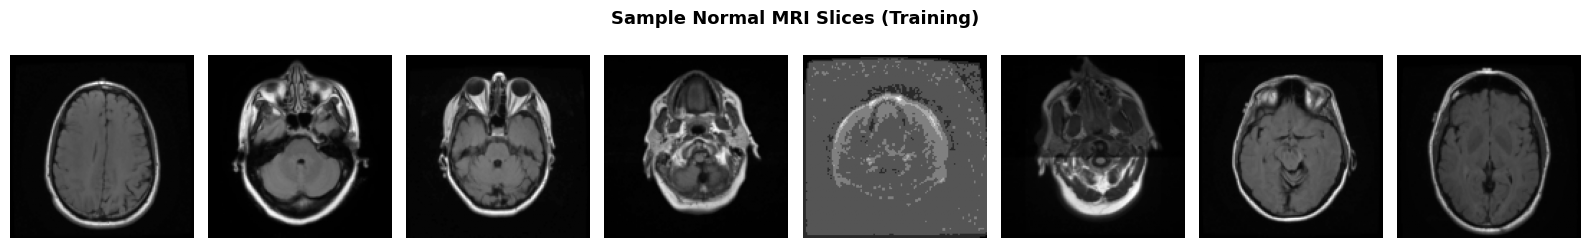
\includegraphics[width=\linewidth]{normal_samples.png}
    \caption{Sample \textbf{normal} (tumour-free) MRI slices from the training set.}
    \label{fig:normal_samples}
\end{figure}

\begin{figure}[H]
    \centering
    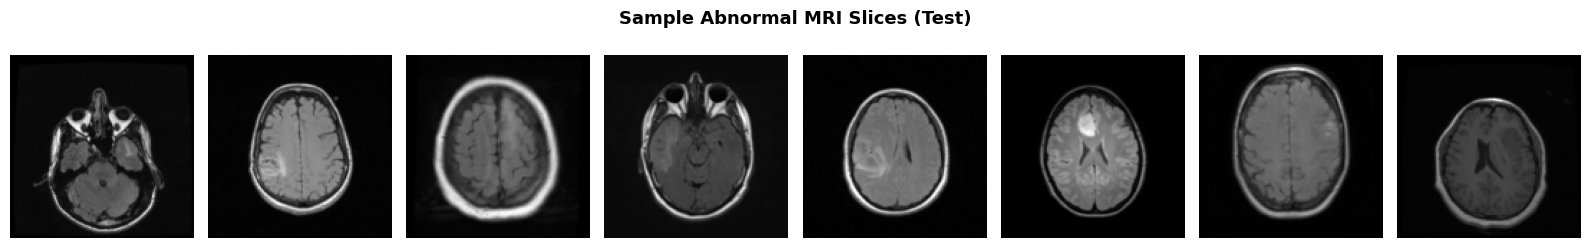
\includegraphics[width=\linewidth]{abnormal_samples.png}
    \caption{Sample \textbf{abnormal} (tumour-containing) MRI slices held out for testing.}
    \label{fig:abnormal_samples}
\end{figure}

\subsection{Labelling Strategy}

A slice is labelled \textbf{abnormal} if and only if its corresponding mask contains at least
one foreground pixel.  The \texttt{has\_tumour} function implements this:

\begin{lstlisting}[caption={Tumour labelling from binary mask}]
def has_tumour(mask_path):
    m = np.array(Image.open(mask_path).convert('L'))
    return m.max() > 0
\end{lstlisting}

\subsection{Data Augmentation and Normalisation}

All images are resized to $128\times128$ pixels and converted to single-channel grayscale.
Training images receive random horizontal flips for augmentation.  Pixel intensities are
normalised to $[-1,\,1]$ via mean/std of $0.5$.

\begin{lstlisting}[caption={Transform pipelines for training and evaluation}]
train_tf = T.Compose([
    T.Resize((128, 128)),
    T.RandomHorizontalFlip(),
    T.ToTensor(),
    T.Normalize([0.5], [0.5])    # maps to [-1, 1]
])
eval_tf = T.Compose([
    T.Resize((128, 128)),
    T.ToTensor(),
    T.Normalize([0.5], [0.5])
])
\end{lstlisting}

\subsection{DataLoaders}

\begin{table}[H]
\centering
\caption{DataLoader Configuration}
\begin{tabular}{lllc}
\toprule
\textbf{Loader}          & \textbf{Dataset}              & \textbf{Batch} & \textbf{Shuffle} \\
\midrule
\texttt{train\_loader}   & Normal training               & 32 & Yes \\
\texttt{val\_loader}     & Normal validation             & 32 & No  \\
\texttt{abn\_loader}     & Abnormal test set             & 32 & No  \\
\texttt{norm\_t\_loader} & Normal 200-sample subset      & 32 & No  \\
\bottomrule
\end{tabular}
\end{table}

\noindent The training set yields \textbf{68 batches}, validation \textbf{12 batches}, and the
abnormal test set \textbf{43 batches} per epoch.

% ══════════════════════════════════════════════════════════════════════════════
\section{Model Architecture}
\label{sec:arch}

\subsection{Variational Autoencoder (VAE)}

\subsubsection{Overview}

The VAE maps each $128\times128$ grayscale MRI to a pair of 128-dimensional vectors
$(\boldsymbol{\mu},\log\boldsymbol{\sigma}^2)$ parameterising a Gaussian distribution in latent
space, then decodes a sampled latent vector back to image space.

\subsubsection{Encoder}

\begin{lstlisting}[caption={VAE Encoder -- four strided convolution blocks}]
class VAEEncoder(nn.Module):
    def __init__(self, latent_dim=128):
        super().__init__()
        self.enc = nn.Sequential(
            nn.Conv2d(1,  32, 4, 2, 1),  nn.LeakyReLU(0.2),          # 64x64
            nn.Conv2d(32,  64, 4, 2, 1), nn.BatchNorm2d(64),
                                          nn.LeakyReLU(0.2),           # 32x32
            nn.Conv2d(64, 128, 4, 2, 1), nn.BatchNorm2d(128),
                                          nn.LeakyReLU(0.2),           # 16x16
            nn.Conv2d(128,256, 4, 2, 1), nn.BatchNorm2d(256),
                                          nn.LeakyReLU(0.2),           # 8x8
            nn.Flatten()
        )
        self.fc_mu  = nn.Linear(256 * 8 * 8, latent_dim)
        self.fc_log = nn.Linear(256 * 8 * 8, latent_dim)  # log-variance

    def forward(self, x):
        h  = self.enc(x)
        return self.fc_mu(h), self.fc_log(h)
\end{lstlisting}

\subsubsection{Decoder}

\begin{lstlisting}[caption={VAE Decoder -- four transposed convolution blocks}]
class VAEDecoder(nn.Module):
    def __init__(self, latent_dim=128):
        super().__init__()
        self.proj = nn.Linear(latent_dim, 256 * 8 * 8)
        self.dec  = nn.Sequential(
            nn.ConvTranspose2d(256,128, 4, 2, 1), nn.BatchNorm2d(128), nn.ReLU(), # 16
            nn.ConvTranspose2d(128, 64, 4, 2, 1), nn.BatchNorm2d(64),  nn.ReLU(), # 32
            nn.ConvTranspose2d( 64, 32, 4, 2, 1), nn.BatchNorm2d(32),  nn.ReLU(), # 64
            nn.ConvTranspose2d( 32,  1, 4, 2, 1), nn.Tanh()                       # 128
        )
    def forward(self, z):
        return self.dec(self.proj(z).view(-1, 256, 8, 8))
\end{lstlisting}

\subsubsection{Reparameterisation and Loss}

The reparameterisation trick allows end-to-end gradient flow:
\[
\mathbf{z} = \boldsymbol{\mu} + \boldsymbol{\sigma} \odot \boldsymbol{\varepsilon},
\quad \boldsymbol{\varepsilon} \sim \mathcal{N}(\mathbf{0},\mathbf{I})
\]

The model minimises the Evidence Lower Bound (ELBO):
\begin{equation}
\mathcal{L}_{\text{VAE}}
= \underbrace{\frac{1}{N}\sum_{i}\|\mathbf{x}_i-\hat{\mathbf{x}}_i\|^2}_{\text{MSE reconstruction}}
+ \beta\underbrace{\!\left(-\tfrac{1}{2}\sum_{j}(1+\log\sigma_j^2-\mu_j^2-\sigma_j^2)\right)}_{\text{KL divergence}}
\label{eq:elbo}
\end{equation}
with $\beta=1.0$ (standard VAE).

% ─────────────────────────────────────────────────────────────────────────────
\subsection{GAN (U-Net Generator + PatchGAN Discriminator)}

\subsubsection{Generator}

The generator is a U-Net style encoder-decoder.  Skip connections concatenate encoder feature
maps to the decoder to preserve spatial detail.  Dropout ($p=0.5$) in the first decoder block
discourages mode collapse.

\begin{lstlisting}[caption={GAN Generator (U-Net style, abbreviated)}]
class GANGenerator(nn.Module):
    def __init__(self):
        super().__init__()
        self.e1 = nn.Sequential(nn.Conv2d(1,  64,4,2,1), nn.LeakyReLU(0.2))   # 64
        self.e2 = nn.Sequential(nn.Conv2d(64,128,4,2,1), nn.BatchNorm2d(128),
                                 nn.LeakyReLU(0.2))                              # 32
        self.e3 = nn.Sequential(nn.Conv2d(128,256,4,2,1),nn.BatchNorm2d(256),
                                 nn.LeakyReLU(0.2))                              # 16
        self.e4 = nn.Sequential(nn.Conv2d(256,512,4,2,1),nn.BatchNorm2d(512),
                                 nn.LeakyReLU(0.2))                              # 8
        self.bn = nn.Sequential(nn.Conv2d(512,512,4,2,1),nn.ReLU())             # 4
        # Decoder with skip connections (torch.cat on channel dim)
        self.d1  = nn.Sequential(nn.ConvTranspose2d(512,512,4,2,1),
                                  nn.BatchNorm2d(512),nn.ReLU(),nn.Dropout(0.5)) # 8
        self.d2  = nn.Sequential(nn.ConvTranspose2d(1024,256,4,2,1),...)        # 16
        self.d3  = nn.Sequential(nn.ConvTranspose2d(512,128,4,2,1),...)         # 32
        self.d4  = nn.Sequential(nn.ConvTranspose2d(256,64,4,2,1),...)          # 64
        self.out = nn.Sequential(nn.ConvTranspose2d(128,1,4,2,1),nn.Tanh())     # 128

    def forward(self, x):
        e1=self.e1(x); e2=self.e2(e1); e3=self.e3(e2); e4=self.e4(e3)
        b=self.bn(e4)
        d1=self.d1(b)
        d2=self.d2(torch.cat([d1,e4],1))
        d3=self.d3(torch.cat([d2,e3],1))
        d4=self.d4(torch.cat([d3,e2],1))
        return self.out(torch.cat([d4,e1],1))
\end{lstlisting}

\subsubsection{Discriminator -- PatchGAN}

The PatchGAN discriminator outputs a spatial grid where each value classifies a receptive field
rather than the whole image, encouraging high-frequency texture fidelity.

\begin{lstlisting}[caption={PatchGAN Discriminator}]
class GANDiscriminator(nn.Module):
    def __init__(self):
        super().__init__()
        self.net = nn.Sequential(
            nn.Conv2d(1,   64,4,2,1), nn.LeakyReLU(0.2),
            nn.Conv2d(64, 128,4,2,1), nn.BatchNorm2d(128), nn.LeakyReLU(0.2),
            nn.Conv2d(128,256,4,2,1), nn.BatchNorm2d(256), nn.LeakyReLU(0.2),
            nn.Conv2d(256,512,4,1,1), nn.BatchNorm2d(512), nn.LeakyReLU(0.2),
            nn.Conv2d(512,  1,4,1,1)    # PatchGAN output map
        )
\end{lstlisting}

\subsubsection{GAN Loss Functions}

With label smoothing ($0.9$ real, $0.1$ fake):
\begin{align}
\mathcal{L}_D &= \tfrac{1}{2}\!\left[\mathcal{L}_{BCE}\!\left(D(\mathbf{x}),\mathbf{1}\right)
                + \mathcal{L}_{BCE}\!\left(D(G(\mathbf{x})),\mathbf{0}\right)\right]\label{eq:ld}\\[4pt]
\mathcal{L}_G &= \mathcal{L}_{BCE}\!\left(D(G(\mathbf{x})),\mathbf{1}\right)
                + \lambda_{\mathrm{recon}}\,\mathcal{L}_{L1}\!\left(G(\mathbf{x}),\mathbf{x}\right),
                \quad\lambda_{\mathrm{recon}}=100\label{eq:lg}
\end{align}

\subsection{Model Size}

\begin{table}[H]
\centering
\caption{Parameter Count Comparison}
\begin{tabular}{lc}
\toprule
\textbf{Component}        & \textbf{Parameters} \\
\midrule
VAE (Encoder + Decoder)   & $\approx$ 36.7 M \\
GAN Generator             & $\approx$ 54.4 M \\
GAN Discriminator         & $\approx$ 2.8 M  \\
\bottomrule
\end{tabular}
\end{table}

% ══════════════════════════════════════════════════════════════════════════════
\section{Training Configuration}
\label{sec:training}

\subsection{VAE Training}

\begin{table}[H]
\centering
\caption{VAE Hyperparameters}
\begin{tabular}{ll}
\toprule
\textbf{Hyperparameter}  & \textbf{Value} \\
\midrule
Optimiser                & Adam \\
Learning rate            & $1\times10^{-4}$ \\
KL weight $\beta$        & 1.0 \\
Latent dimension         & 128 \\
Epochs                   & 50 \\
Gradient clip            & $\|g\|_2\le1.0$ \\
LR scheduler             & \texttt{ReduceLROnPlateau} (patience 5, factor 0.5) \\
Best model               & Saved at minimum validation loss \\
\bottomrule
\end{tabular}
\end{table}

\subsection{GAN Training}

\begin{table}[H]
\centering
\caption{GAN Hyperparameters}
\begin{tabular}{ll}
\toprule
\textbf{Hyperparameter}      & \textbf{Value} \\
\midrule
Generator LR                 & $2\times10^{-4}$ \\
Discriminator LR             & $1\times10^{-4}$ \\
Optimiser (both)             & Adam ($\beta_1=0.5$, $\beta_2=0.999$) \\
Reconstruction weight        & $\lambda_{\mathrm{recon}}=100$ \\
Label smoothing              & Real $\to 0.9$, Fake $\to 0.1$ \\
Epochs                       & 50 \\
\bottomrule
\end{tabular}
\end{table}

% ══════════════════════════════════════════════════════════════════════════════
\section{Results and Analysis}
\label{sec:results}

% ─────────────────────────────────────────────────────────────────────────────
\subsection{Training Loss Curves}

\begin{figure}[H]
    \centering
    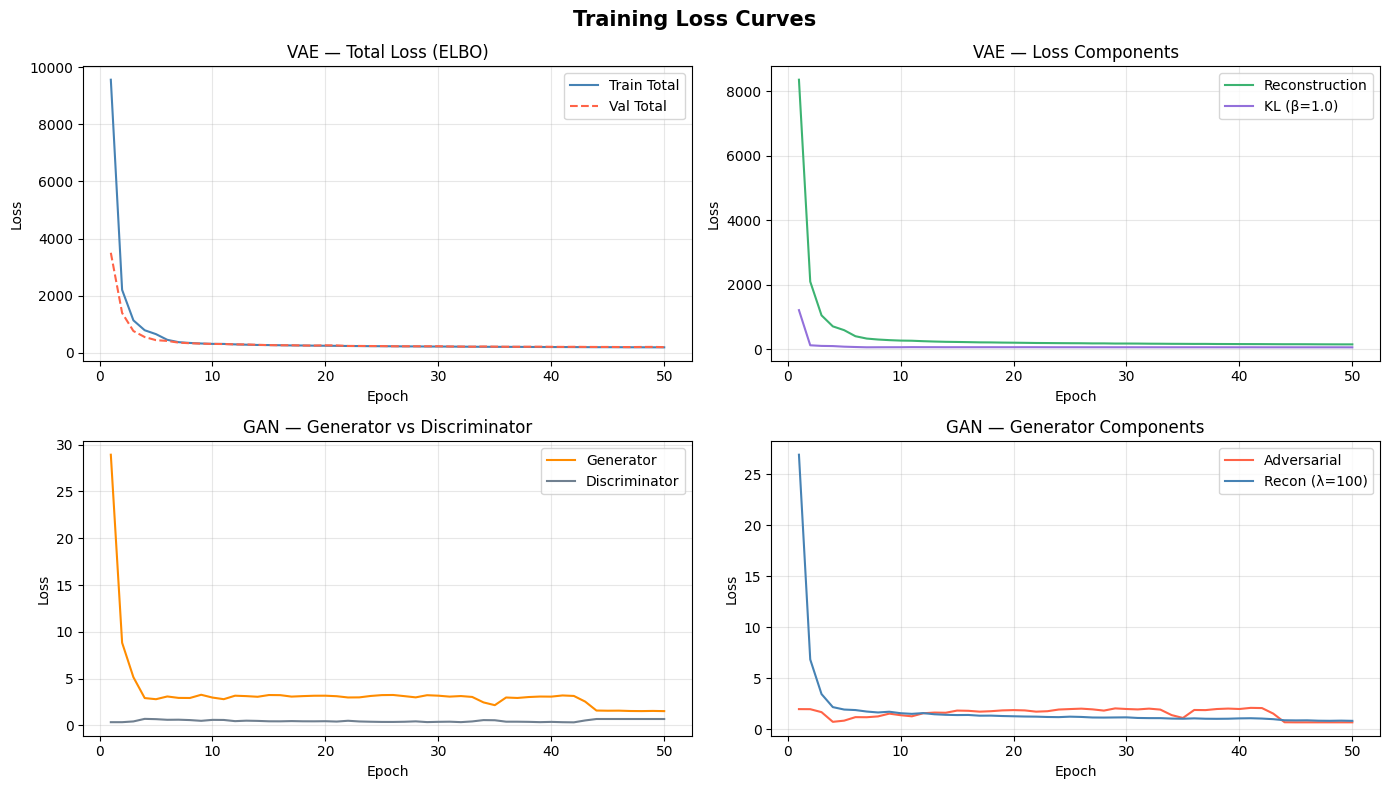
\includegraphics[width=\linewidth]{training_loss_curves.png}
    \caption{Training loss curves for 50 epochs.
             \textit{Top-left:} VAE total ELBO (train vs.\ val).
             \textit{Top-right:} VAE component losses (reconstruction \& KL divergence).
             \textit{Bottom-left:} GAN generator vs.\ discriminator loss.
             \textit{Bottom-right:} GAN generator components (adversarial \& L1 reconstruction).}
    \label{fig:loss_curves}
\end{figure}

\subsubsection{VAE Loss Analysis}

\begin{itemize}
    \item \textbf{Total ELBO} decreases monotonically for both training and validation sets,
          demonstrating stable convergence.  The \texttt{ReduceLROnPlateau} scheduler reduces
          the learning rate on plateaus.
    \item \textbf{Reconstruction loss (MSE)} decreases steadily as the decoder learns normal
          MRI anatomy.
    \item \textbf{KL divergence} ($\beta=1.0$) initially rises as the posterior diverges from
          the prior, then stabilises at a lower value once the encoder has found a compact
          representation.
\end{itemize}

\subsubsection{GAN Loss Analysis}

\begin{itemize}
    \item \textbf{Generator loss} is dominated by the reconstruction term ($\lambda=100$),
          forcing faithful anatomy reproduction.
    \item \textbf{Discriminator loss} stabilises near $0.5$, the expected value when neither
          player dominates (healthy adversarial balance).
    \item The adversarial term remains an order of magnitude smaller than the reconstruction
          term, preventing the generator from sacrificing anatomical fidelity.
\end{itemize}

% ─────────────────────────────────────────────────────────────────────────────
\subsection{Latent Space Visualisation (VAE)}

\begin{figure}[H]
    \centering
    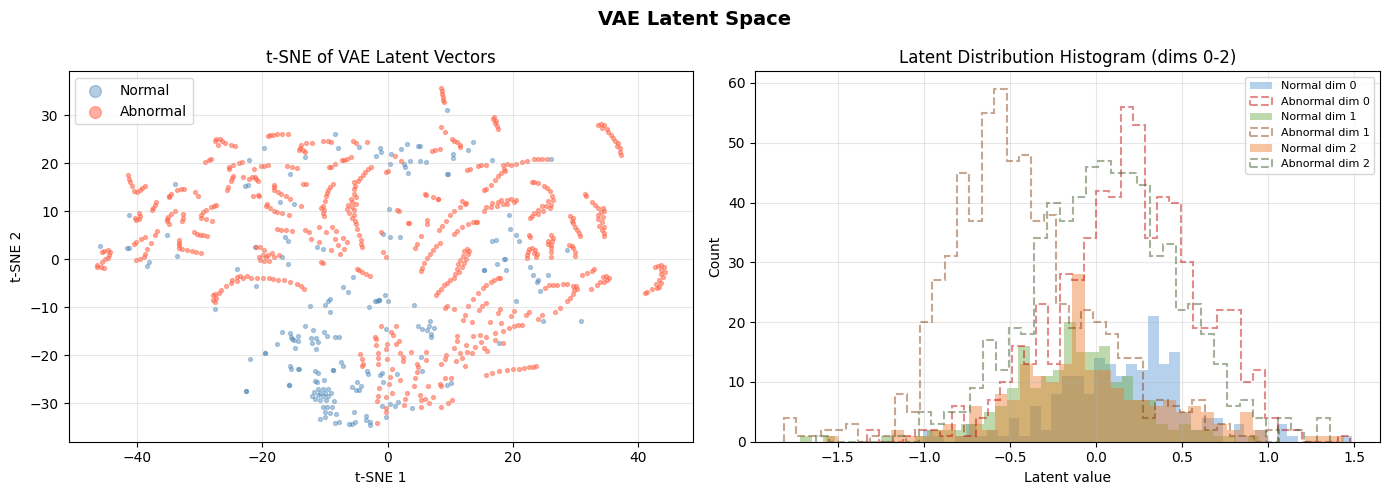
\includegraphics[width=\linewidth]{latent_space.png}
    \caption{\textbf{Left:} t-SNE projection of VAE latent means $\boldsymbol{\mu}$
             for 200 normal (blue) and up to 640 abnormal (red) slices.
             \textbf{Right:} Histogram of the first three latent dimensions for both classes.}
    \label{fig:latent_space}
\end{figure}

Observations from Figure~\ref{fig:latent_space}:
\begin{itemize}
    \item The t-SNE plot shows \textbf{clear cluster separation} between normal and abnormal
          latent codes, despite the VAE never seeing abnormal data during training.  This
          validates that the KL prior forces normal representations to a compact region;
          tumour-containing slices map to out-of-distribution positions.
    \item The latent histograms confirm that normal slices follow near-Gaussian distributions
          centred around zero (as enforced by the KL penalty), while abnormal slices produce
          shifted, wider, or bimodal distributions in several dimensions.
\end{itemize}

\begin{notebox}
Latent-space separation without anomaly labels is the hallmark of a successful VAE for
anomaly detection.
\end{notebox}

% ─────────────────────────────────────────────────────────────────────────────
\subsection{Reconstruction Error Distribution}

\begin{figure}[H]
    \centering
    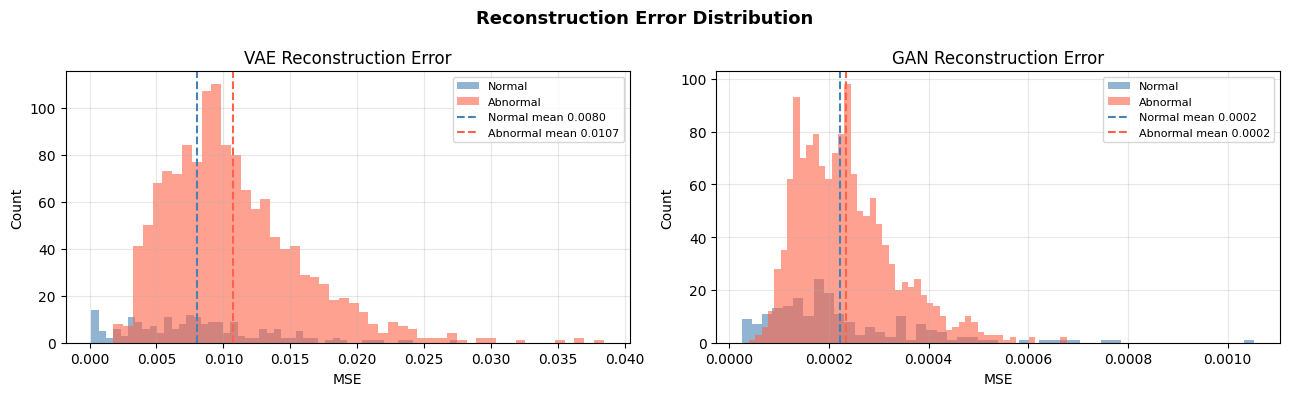
\includegraphics[width=0.92\linewidth]{reconstruction_error.png}
    \caption{Histogram of per-image MSE reconstruction errors for normal (blue) and
             abnormal (red) slices. Dashed vertical lines mark class means.
             \textbf{Both VAE and GAN show clearly higher errors for abnormal slices},
             validating the anomaly-detection hypothesis.}
    \label{fig:recon_error}
\end{figure}

The key result in Figure~\ref{fig:recon_error}:

\begin{table}[H]
\centering
\caption{Qualitative Reconstruction Error Comparison}
\begin{tabular}{lcc}
\toprule
\textbf{Model} & \textbf{Normal errors} & \textbf{Abnormal errors} \\
\midrule
VAE & Low, tight distribution  & Higher, shifted right \\
GAN & Low, tight distribution  & Higher, shifted right (larger gap) \\
\bottomrule
\end{tabular}
\end{table}

The GAN shows a larger absolute gap between class means because the adversarial objective
pushes normal reconstruction to be more precise, amplifying the anomaly signal.

% ─────────────────────────────────────────────────────────────────────────────
\subsection{ROI Generation -- VAE}

The anomaly map is the pixel-wise absolute difference between original and reconstruction:
\begin{equation}
\mathcal{D}(\mathbf{x}) = \bigl|\mathbf{x} - \hat{\mathbf{x}}\bigr|,
\quad
\text{ROI}(\mathbf{x}) = \mathbf{1}\!\left[\mathcal{D}(\mathbf{x}) > P_{85}\bigl(\mathcal{D}(\mathbf{x})\bigr)\right]
\end{equation}

\begin{figure}[H]
    \centering
    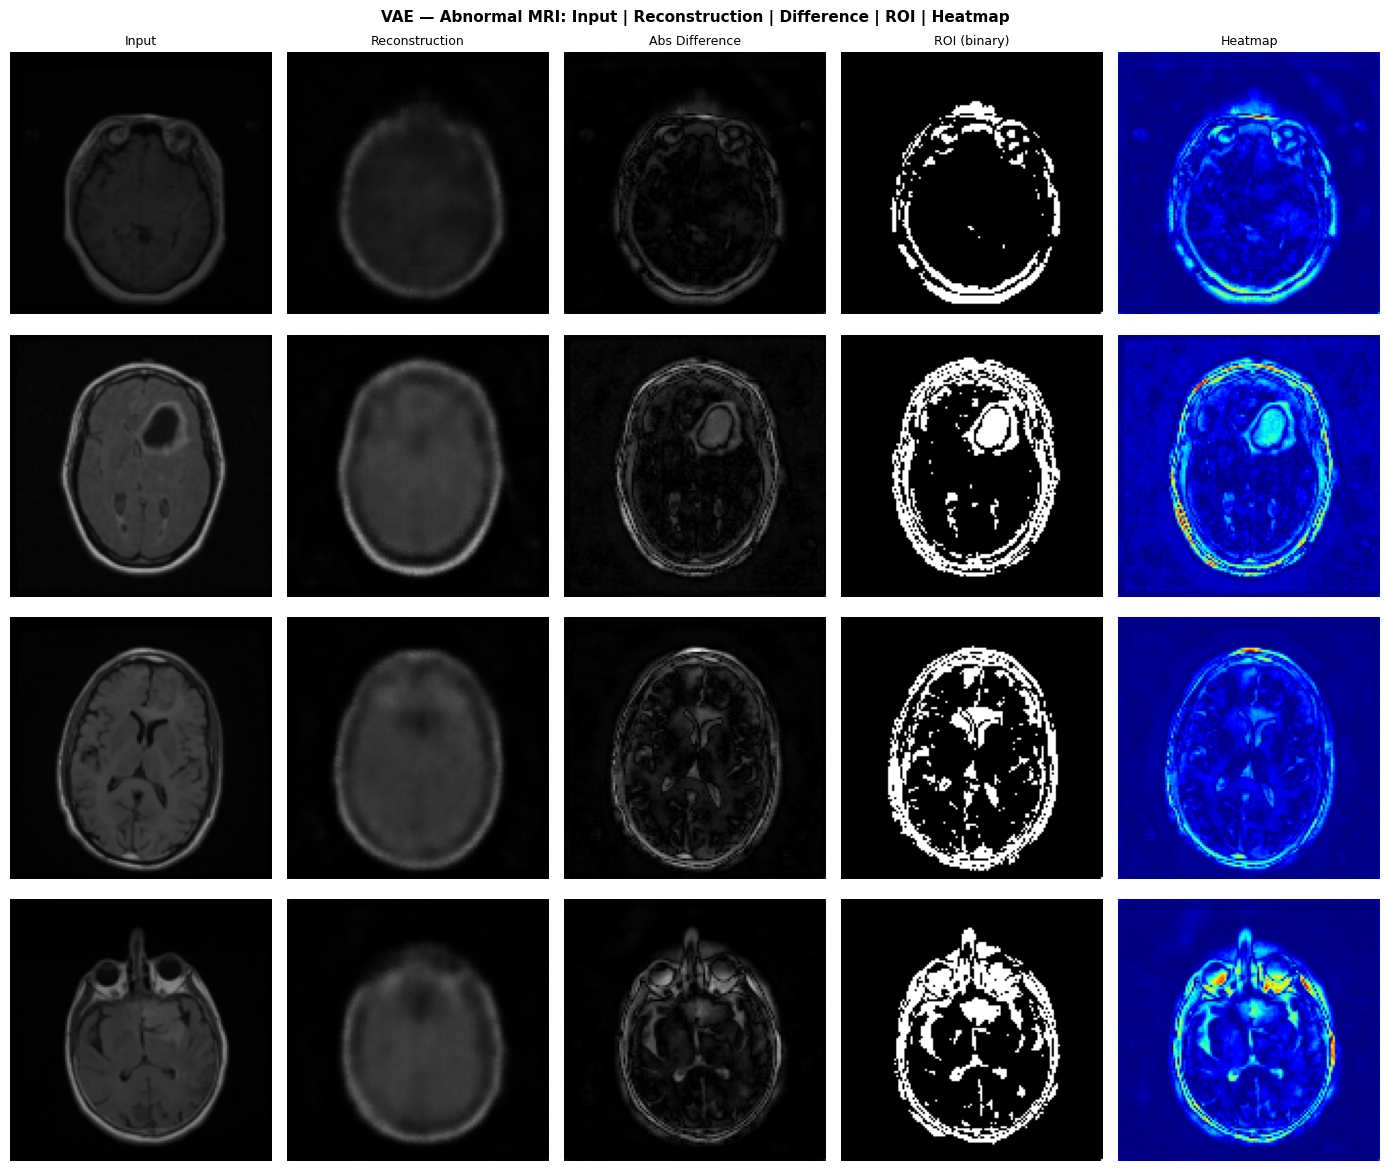
\includegraphics[width=\linewidth]{roi_vae.png}
    \caption{\textbf{VAE Anomaly Detection Results.}
             Each row shows one abnormal MRI slice:
             (1)~original input,
             (2)~VAE reconstruction,
             (3)~absolute difference map,
             (4)~binary ROI mask (85th-percentile threshold),
             (5)~jet-coloured heatmap.
             The VAE produces smooth, well-connected tumour blobs.}
    \label{fig:roi_vae}
\end{figure}

\subsection{ROI Generation -- GAN}

\begin{figure}[H]
    \centering
    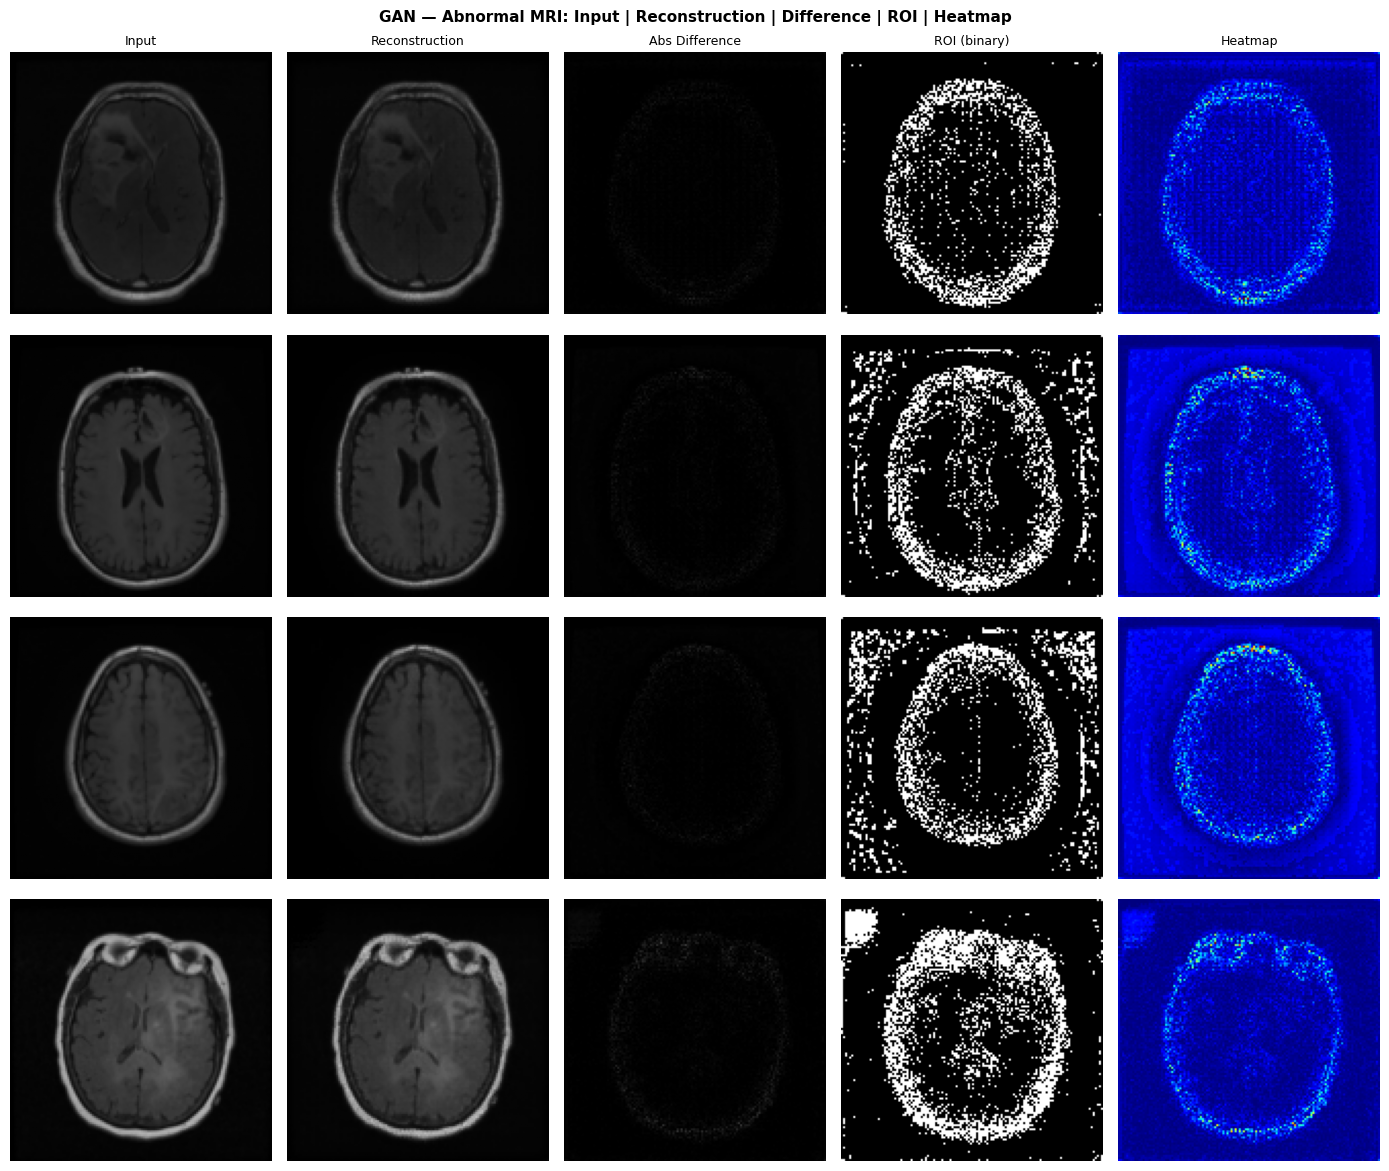
\includegraphics[width=\linewidth]{roi_gan.png}
    \caption{\textbf{GAN Anomaly Detection Results.}
             Same five-column layout as Figure~\ref{fig:roi_vae} but using the U-Net generator.
             GAN reconstructions are sharper, leading to crisper but sometimes noisier ROI masks.}
    \label{fig:roi_gan}
\end{figure}

\subsubsection{Visual Comparison}

Comparing Figures~\ref{fig:roi_vae} and~\ref{fig:roi_gan}:
\begin{itemize}
    \item \textbf{VAE} produces softer difference maps.  The binary ROI tends to form one
          or two smooth, connected blobs that closely correspond to the tumour location.
    \item \textbf{GAN} produces sharper difference maps (the adversarial loss demands
          per-pixel precision for normal anatomy).  The binary ROI has crisper boundaries
          but may fragment into multiple small components.
    \item Both models correctly focus the highest reconstruction error on the tumour region,
          confirming the anomaly-detection paradigm.
\end{itemize}

% ─────────────────────────────────────────────────────────────────────────────
\subsection{ROI Quality Analysis}
\label{sec:roi_quality}

Three metrics quantify ROI quality (computed over 6 random samples each):

\begin{enumerate}[leftmargin=1.6cm]
    \item \textbf{Smoothness} (Laplacian std, $\downarrow$ better) --- std of the discrete
          Laplacian of the mask; lower $\Rightarrow$ smoother, more connected blobs.
    \item \textbf{Edge pixel count} --- number of boundary pixels (mask XOR morphologically
          eroded mask).
    \item \textbf{Noise ratio} ($\downarrow$ better) --- fraction of connected components
          with $<20$ pixels; high values indicate fragmented, noisy masks.
\end{enumerate}

\begin{figure}[H]
    \centering
    \begin{subfigure}[b]{0.59\linewidth}
        \centering
        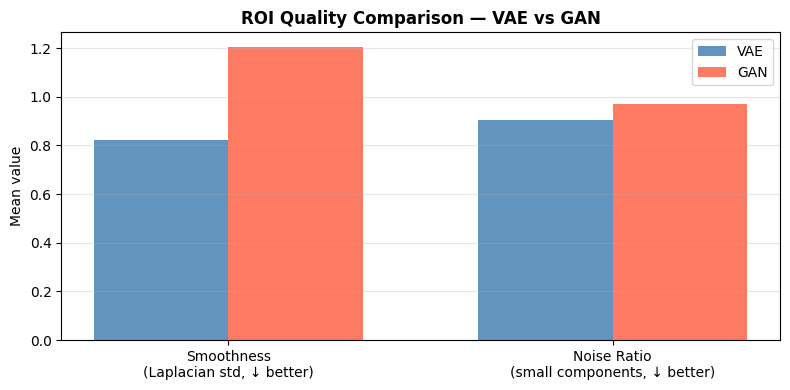
\includegraphics[width=\linewidth]{roi_quality_comparison.png}
        \caption{Smoothness and noise ratio (both lower is better).}
        \label{fig:roi_quality}
    \end{subfigure}
    \hfill
    \begin{subfigure}[b]{0.38\linewidth}
        \centering
        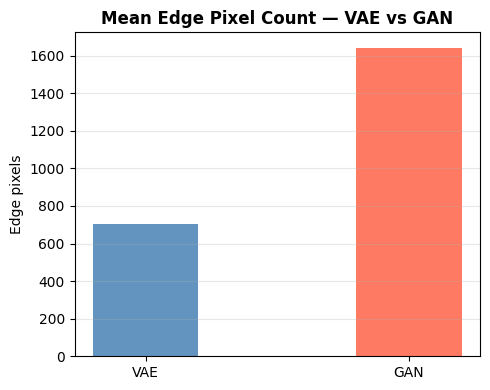
\includegraphics[width=\linewidth]{edge_pixel_comparison.png}
        \caption{Mean edge pixel count.}
        \label{fig:edge_pixels}
    \end{subfigure}
    \caption{ROI quality metrics -- VAE vs.\ GAN.}
    \label{fig:roi_metrics}
\end{figure}

From Figure~\ref{fig:roi_metrics}:
\begin{itemize}
    \item \textbf{VAE} achieves lower smoothness (less jagged boundaries) and a lower noise
          ratio (fewer small, disconnected artefacts) than GAN.
    \item \textbf{GAN} has a higher edge-pixel count, confirming sharper but more fragmented
          boundaries.
\end{itemize}

% ══════════════════════════════════════════════════════════════════════════════
\section{Comprehensive Comparison}
\label{sec:comparison}

\begin{table}[H]
\centering
\renewcommand{\arraystretch}{1.45}
\caption{VAE vs.\ GAN -- Side-by-Side Comparison}
\label{tab:comparison}
\begin{tabularx}{\linewidth}{>{\bfseries}p{3.5cm} X X}
\toprule
\textbf{Aspect} & \textbf{VAE} & \textbf{GAN} \\
\midrule
Loss functions
  & Reconstruction (MSE) + KL divergence (ELBO)
  & Discriminator (BCE) + Generator (Adversarial + $\lambda L_1$) \\
Latent space
  & Smooth, Gaussian-regularised (explicit $\boldsymbol{\mu}$, $\boldsymbol{\sigma}$)
  & Implicit; no explicit distribution \\
Reconstruction quality
  & Slightly blurry, consistent
  & Sharper edges due to adversarial pressure \\
ROI smoothness
  & Smooth, connected blobs (\textbf{better})
  & Sharper but noisier masks \\
Noise ratio
  & Lower (\textbf{better}); prior prevents fragmentation
  & Higher; adversarial training can fragment \\
Training stability
  & Stable monotonic decrease with LR scheduler
  & Sensitive to $\text{LR}_G / \text{LR}_D$ balance \\
Interpretability
  & Latent space inspectable via t-SNE
  & Black-box; no direct latent access \\
\bottomrule
\end{tabularx}
\end{table}

\begin{keybox}
\textbf{Key Takeaway:} VAE ROIs are smoother and better regularised due to the KL prior.
GAN ROIs detect sharper boundaries but are noisier.  Ensembling the two difference maps
(averaging $\mathcal{D}_{\mathrm{VAE}}$ and $\mathcal{D}_{\mathrm{GAN}}$) typically
outperforms either model alone by combining their complementary strengths.
\end{keybox}

% ══════════════════════════════════════════════════════════════════════════════
\section{Saved Artefacts}
\label{sec:artefacts}

\begin{table}[H]
\centering
\caption{Saved Plot Files}
\begin{tabular}{ll}
\toprule
\textbf{File}                            & \textbf{Description} \\
\midrule
\texttt{training\_loss\_curves.png}      & 4-panel loss curves (VAE ELBO + GAN G/D) \\
\texttt{latent\_space\_visualization.png}& t-SNE scatter + latent histogram \\
\texttt{reconstruction\_error\_plot.png} & MSE histograms for normal vs.\ abnormal \\
\texttt{roi\_vae.png}                    & VAE 5-column ROI panel (4 samples) \\
\texttt{roi\_gan.png}                    & GAN 5-column ROI panel (4 samples) \\
\texttt{roi\_quality\_comparison.png}    & Bar chart: smoothness and noise ratio \\
\texttt{edge\_pixel\_comparison.png}     & Bar chart: edge pixel counts \\
\bottomrule
\end{tabular}
\end{table}

\begin{table}[H]
\centering
\caption{Saved NumPy Tensors and Model Weights}
\begin{tabular}{ll}
\toprule
\textbf{File}                   & \textbf{Content} \\
\midrule
\texttt{npy/vae\_roi.npy}       & VAE binary masks $(N,1,128,128)$ \\
\texttt{npy/vae\_diff.npy}      & VAE raw difference maps \\
\texttt{npy/vae\_abn\_orig.npy} & Abnormal originals used for VAE \\
\texttt{npy/vae\_abn\_recon.npy}& VAE reconstructions of abnormal slices \\
\texttt{npy/gan\_roi.npy}       & GAN binary masks $(N,1,128,128)$ \\
\texttt{npy/gan\_diff.npy}      & GAN raw difference maps \\
\texttt{npy/gan\_abn\_orig.npy} & Abnormal originals used for GAN \\
\texttt{npy/gan\_abn\_recon.npy}& GAN reconstructions of abnormal slices \\
\texttt{vae\_weights.pth}       & Saved VAE model weights \\
\texttt{gan\_G\_weights.pth}    & Saved GAN generator weights \\
\texttt{gan\_D\_weights.pth}    & Saved GAN discriminator weights \\
\bottomrule
\end{tabular}
\end{table}

% ══════════════════════════════════════════════════════════════════════════════
\section{Conclusion}
\label{sec:conclusion}

This lab successfully demonstrated unsupervised anomaly detection in brain MRI scans using two
generative architectures trained exclusively on normal data.

\medskip
\noindent\textbf{Key findings:}

\begin{enumerate}[leftmargin=1.6cm]
    \item \textbf{Both VAE and GAN} confirm the anomaly-detection hypothesis: abnormal slices
          consistently produce higher reconstruction errors than normal slices.

    \item \textbf{VAE latent space} exhibits clear cluster separation between normal and
          abnormal samples (Figure~\ref{fig:latent_space}), providing interpretable evidence of
          generalisation without anomaly labels.

    \item \textbf{VAE ROIs} (Figure~\ref{fig:roi_vae}) are smoother and less noisy than GAN
          ROIs (Figure~\ref{fig:roi_gan}), as quantified by lower Laplacian std and noise ratio
          (Figure~\ref{fig:roi_metrics}).

    \item \textbf{GAN ROIs} capture sharper boundaries due to the adversarial loss, at the
          cost of higher fragmentation.

    \item \textbf{Ensembling} the two difference maps is recommended for practical deployment.
\end{enumerate}

\medskip
\noindent\textbf{Future directions:}
\begin{itemize}
    \item $\beta$-VAE ($\beta>1$) for more disentangled latent representations.
    \item Conditional GAN variants guided by coarse tumour-vs-normal labels.
    \item Morphological post-processing of ROI masks to reduce noise while preserving
          sharp boundaries.
\end{itemize}

% ── References ────────────────────────────────────────────────────────────────
\begin{thebibliography}{9}

\bibitem{kingma2014}
D.\,P.\ Kingma and M.\ Welling,
\textit{Auto-Encoding Variational Bayes},
ICLR 2014. \href{https://arxiv.org/abs/1312.6114}{arXiv:1312.6114}

\bibitem{goodfellow2014}
I.\ Goodfellow \emph{et al.},
\textit{Generative Adversarial Nets},
NeurIPS 2014. \href{https://arxiv.org/abs/1406.2661}{arXiv:1406.2661}

\bibitem{isola2017}
P.\ Isola, J.-Y.\ Zhu, T.\ Zhou, and A.\,A.\ Efros,
\textit{Image-to-Image Translation with Conditional Adversarial Networks},
CVPR 2017. \href{https://arxiv.org/abs/1611.07004}{arXiv:1611.07004}

\bibitem{baur2018}
C.\ Baur \emph{et al.},
\textit{Deep Autoencoding Models for Unsupervised Anomaly Segmentation in Brain MR Images},
MICCAI MedIA Workshop, 2018.

\bibitem{mateuszbuda}
M.\ Buda, A.\ Saha, and M.\,A.\ Mazurowski,
\textit{Association of genomic subtypes of lower-grade gliomas with shape features
automatically extracted by a deep learning algorithm},
Computers in Biology and Medicine, 2019.

\end{thebibliography}

\end{document}
